\documentclass[12pt]{article} 
\usepackage[margin=1in]{geometry}
\usepackage{tikz,amsmath}

\begin{document}

% graph01.png
$$
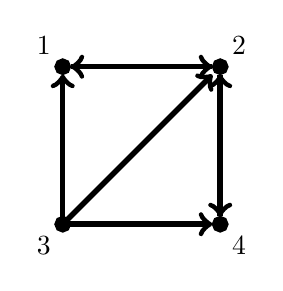
\begin{tikzpicture}[scale=2.0,line width=2pt]
\filldraw (0,0) circle (1pt); \filldraw (0,1) circle (1pt);
\filldraw (1,1) circle (1pt); \filldraw (1,0) circle (1pt);
\draw (0,1) node[anchor=south east] {1};
\draw (1,1) node[anchor=south west] {2};
\draw (1,0) node[anchor=north west] {4};
\draw (0,0) node[anchor=north east] {3};
\draw [->] (0,0) to (0,0.95);
\draw [->] (0,0) to (0.95,0);
\draw [->] (0,0) to (0.95,0.95);
\draw [->] (1,0.95) to (1,0.05);
\draw [->] (1,0.05) to (1,0.95);
\draw [->] (0.05,1) to (0.95,1);
\draw [->] (0.95,1) to (0.05,1);
\end{tikzpicture}
$$

% graph02.png
$$
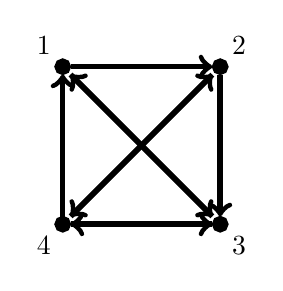
\begin{tikzpicture}[scale=2.0,line width=2pt]
\filldraw (0,0) circle (1pt); \filldraw (0,1) circle (1pt);
\filldraw (1,1) circle (1pt); \filldraw (1,0) circle (1pt);
\draw (0,1) node[anchor=south east] {1};
\draw (1,1) node[anchor=south west] {2};
\draw (1,0) node[anchor=north west] {3};
\draw (0,0) node[anchor=north east] {4};
\draw [->] (0,0) to (0,0.95);
\draw [->] (0.05,0) to (0.95,0);
\draw [->] (0.95,0) to (0.05,0);
\draw [->] (0.05,0.05) to (0.95,0.95);
\draw [->] (0.95,0.95) to (0.05,0.05);
\draw [->] (0.05,0.95) to (0.95,0.05);
\draw [->] (0.95,0.05) to (0.05,0.95);
\draw [->] (1,0.95) to (1,0.05);
\draw [->] (0.05,1) to (0.95,1);

%\draw [->] (0.05,1.05) to[out=45,in=135] (0.95,1.07);
%\draw [->] (0.05,1) to[out=0,in=90] (1,0.1);
%\draw [->] (0.95,0) to[out=180,in=-90] (0,0.9);
%\draw [->] (0.05,0.05) to[out=45,in=135] (0.9,0.05);
%\draw [->] (0.95,-0.05) to[in=-45,out=225] (0.07,-0.07);
%\draw [->] (-0.05,0.05) to[out=135,in=225] (-0.1,0.95);
%\draw [->] (1.05,0.95) to[out=-45,in=45] (1.1,0.05);
%\draw [->] (0,0.05) to[out=90,in=180] (0.9,1);
%\draw [->] (1,0.95) to[out=-90,in=0] (0.1,0);
\end{tikzpicture}
$$

% stem01.png
$$
\begin{tikzpicture}
\draw [->] (0,0) -- (8,0) node[below right] {$n$}; \draw [->] (0,-1.5) -- (0,1.5) node[above left] {$\boldsymbol{x}[n]$};
\draw (0.1,1) -- (-0.1,1) node[left] {1}; \draw (0.1,-1) -- (-0.1,-1) node[left] {$-1$};
\foreach \x/\y in { 0/1 , 1/0.7071 , 2/0 , 3/-0.7071 , 4/-1 , 5/-0.7071 , 6/0 , 7/0.7071} { \filldraw (\x,0) -- (\x,\y) circle[radius=2pt]; }
\foreach \k in {0,...,7} { \draw (\k,0) node[below right] {$\k$}; }
\end{tikzpicture}
$$

% stem02.png
$$
\begin{tikzpicture}
\draw [->] (0,0) -- (8,0) node[below right] {$n$}; \draw [->] (0,-1.5) -- (0,1.5) node[above left] {$\boldsymbol{x}[n]$};
\draw (0.1,1) -- (-0.1,1) node[left] {1}; \draw (0.1,-1) -- (-0.1,-1) node[left] {$-1$};
\foreach \x/\y in { 0/1 , 1/0 , 2/-1 , 3/0 , 4/1 , 5/0 , 6/-1 , 7/0} { \filldraw (\x,0) -- (\x,\y) circle[radius=2pt]; }
\foreach \k in {0,...,7} { \draw (\k,0) node[below right] {$\k$}; }
\end{tikzpicture}
$$

% stem03.png
$$
\begin{tikzpicture}
\draw [->] (0,0) -- (8,0) node[below right] {$n$}; \draw [->] (0,0) -- (0,1.5) node[above left] {$| \boldsymbol{y}[n] |$};
\draw (0.1,1) -- (-0.1,1) node[left] {4}; \draw (0.1,0.5) -- (-0.1,0.5) node[left] {2};
\foreach \x/\y in { 0/0 , 1/1 , 2/0 , 3/0 , 4/0 , 5/0 , 6/0 , 7/1 } { \filldraw (\x,0) -- (\x,\y) circle[radius=2pt]; };
\foreach \k in {0,...,7} { \draw (\k,0) node[below right] {$\k$}; };
\end{tikzpicture}
$$

% stem04.png
$$
\begin{tikzpicture}
\draw [->] (0,0) -- (8,0) node[below right] {$n$}; \draw [->] (0,-1.5) -- (0,1.5) node[above left] {$\angle \boldsymbol{y}[n] $};
\draw (0.1,1) -- (-0.1,1) node[left] {$\pi/2$}; \draw (0.1,-1) -- (-0.1,-1) node[left] {$-\pi/2$};
\foreach \x/\y in { 0/0 , 1/-1 , 2/0 , 3/0 , 4/0 , 5/0 , 6/0 , 7/1 } { \filldraw (\x,0) -- (\x,\y) circle[radius=2pt]; };
\foreach \k in {0,...,7} { \draw (\k,0) node[below right] {$\k$}; };
\end{tikzpicture}
$$

% stem05.png
$$
\begin{tikzpicture}
\draw [->] (0,0) -- (8,0) node[below right] {$n$}; \draw [->] (0,-1.5) -- (0,1.5) node[above left] {$\boldsymbol{x}[n]$};
\draw (0.1,1) -- (-0.1,1) node[left] {1}; \draw (0.1,-1) -- (-0.1,-1) node[left] {$-1$};
\foreach \x/\y in { 0/1 , 1/1 , 2/1 , 3/1 , 4/-1 , 5/-1 , 6/-1 , 7/-1 } { \filldraw (\x,0) -- (\x,\y) circle[radius=2pt]; };
\foreach \k in {0,...,7} { \draw (\k,0) node[below right] {$\k$}; };
\end{tikzpicture}
$$

% stem06.png
$$
\begin{tikzpicture}
\draw [->] (0,0) -- (8,0) node[below right] {$n$}; \draw [->] (0,0) -- (0,2.5) node[above left] {$| \boldsymbol{y}[n] |$};
\draw (0.1,2) -- (-0.1,2) node[left] {6}; \draw (0.1,1) -- (-0.1,1) node[left] {3};
\foreach \x/\y in { 0/0 , 1/1.742 , 2/0 , 3/0.7216 , 4/0 , 5/0.7216 , 6/0 , 7/1.742 } { \filldraw (\x,0) -- (\x,\y) circle[radius=2pt]; };
\foreach \k in {0,...,7} { \draw (\k,0) node[below right] {$\k$}; };
\end{tikzpicture}
$$

% stem07.png
$$
\begin{tikzpicture}
\draw [->] (0,0) -- (8,0) node[below right] {$n$}; \draw [->] (0,-2.5) -- (0,2.5) node[above left] {$\angle \boldsymbol{y}[n] $};
\draw (0.1,2) -- (-0.1,2) node[left] {$\pi/2$}; \draw (0.1,-2) -- (-0.1,-2) node[left] {$-\pi/2$};
\draw (0.1,1) -- (-0.1,1) node[left] {$\pi/4$}; \draw (0.1,-1) -- (-0.1,-1) node[left] {$-\pi/4$};
\foreach \x/\y in { 0/0 , 1/-1.5 , 2/0 , 3/-0.5 , 4/0 , 5/0.5 , 6/0 , 7/1.5 } { \filldraw (\x,0) -- (\x,\y) circle[radius=2pt]; };
\foreach \k in {0,...,7} { \draw (\k,0) node[below right] {$\k$}; };
\end{tikzpicture}
$$

% complex01.png
\begin{tikzpicture}[scale=2]
\draw [->] (-1,0) -- (1,0) node[right] {Re};
\draw [->] (0,-0.5) -- (0,1) node[above] {Im};
\filldraw (0.8,0.8) circle (1pt) node[right] {$z = a + ib$};
\draw[dashed] (0,0.8) -- (0.8,0.8) -- (0.8,0);
\draw[dashed] (0,0) -- (0.8,0.8) node[pos=0.5,above] {$r$};
\draw (0.4,0) node[below right] {$a$};
\draw (0.8,0.4) node[right] {$b$};
\draw (0.3,0.14) node {$\theta$};
\end{tikzpicture}

\end{document}  